\documentclass[letterpaper,12pt]{article}
\usepackage{tabularx} % extra features for tabular environment
\usepackage{amsmath}  % improve math presentation
\usepackage{amsfonts,amssymb}
\usepackage{graphicx} % takes care of graphic including machinery
\usepackage[margin=1in,letterpaper]{geometry} % decreases margins
\usepackage{cite} % takes care of citations
\usepackage[final]{hyperref} % adds hyper links inside the generated pdf file
\usepackage{leftidx}
\usepackage{enumerate}
\usepackage{paralist}
\usepackage{subfigure}
\hypersetup{
	colorlinks=true,       % false: boxed links; true: colored links
	linkcolor=blue,        % color of internal links
	citecolor=blue,        % color of links to bibliography
	filecolor=magenta,     % color of file links
	urlcolor=blue         
}


\begin{document}

\title{Review on Formation Control and Motion Planning for Multi Agents}
\author{Liu Xiangyu}
\date{\today}
\maketitle

\section{Introduction}

The purpose of this article is to briefly introduce the related work on formation control and motion planning for multi agents, for a quick start on our research on formation control via reinforcement learning. In this review, complicated mathmatical details are omitted since detailed mathmatical deduction is not in the scope of this review. 

The organisation of this review is as follows. Section 2,3 and 4 are basically a brief version of the survey of Liu in \cite{liu_bucknall_2018}. Section 5 reviewed some recent works on formation control algorithms using reinforcement learning.

\section{Relationship between Formation Control and Cooperative Motion Planning }

Relationship is illustrated in Figure \ref{fig:CompFcCmp}, details later.

\begin{figure}
	\centering
	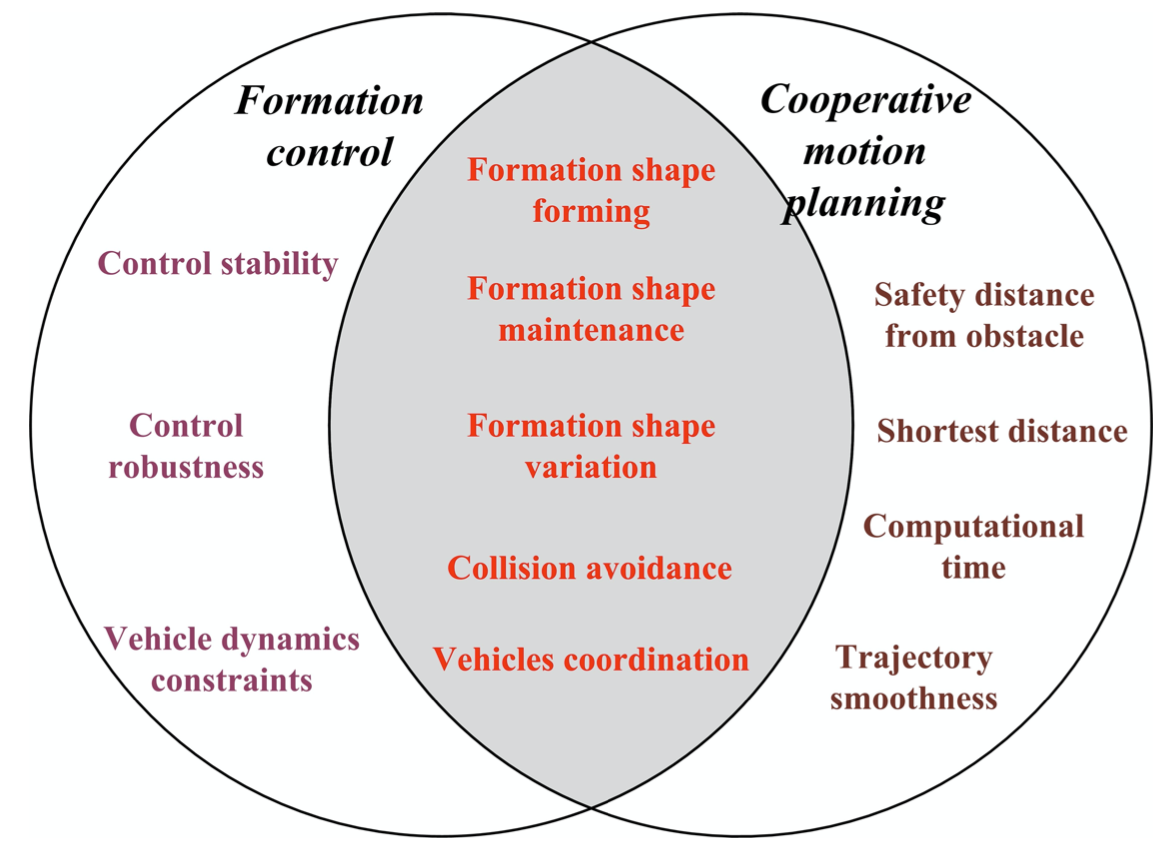
\includegraphics[width=5in]{WX20200510-222400@2x.png}
	\caption{Comparison of formation control and cooperative motion planning \cite{liu_bucknall_2018}.}
	\label{fig:CompFcCmp} 
\end{figure}

\section{Formation Control}

\subsection{System Architecture of Multi Agents Formation}

A generic hierarchical architecture formation system is proposed by Liu and Bucknall in \cite{LIU2015126}. The system is displayed in Figure \ref{fig:FormationSystemArchitecture}, which consists of three layers, i.e. Task Management Layer, Path Planning Layer and Task Execution Layer. According to Liu and Bucknall, the first layer Task Management Layer allocates mission to indivisual vehicles based upon the critiria of maximum overall performance and minimum mission time. In other words, this layer analyzes the mission, which can be defined as a set of waypoints including starting and ending points, and design a proper formation shape, and allocate the formation information to each vehicle.

The Path Planning Layer is comprised of three sub modules, which can concluded as,

\begin{compactenum}
	\item Cooperative path planning module. This is the core of the system, determining the optimised path for each vehicle.
	\item Real-time trajectory modification module. The calculated optimised path is furthur modificated in this module considering the uncertainties in practical applications.
	\item Data acquisition module.
\end{compactenum}

The last module i.e. Task Execution Layer is the execution layer that directly connects to the controllers of vehicles. And execution results are fed back to upper layer to generate a closed loop control.

\begin{figure}
	\centering
	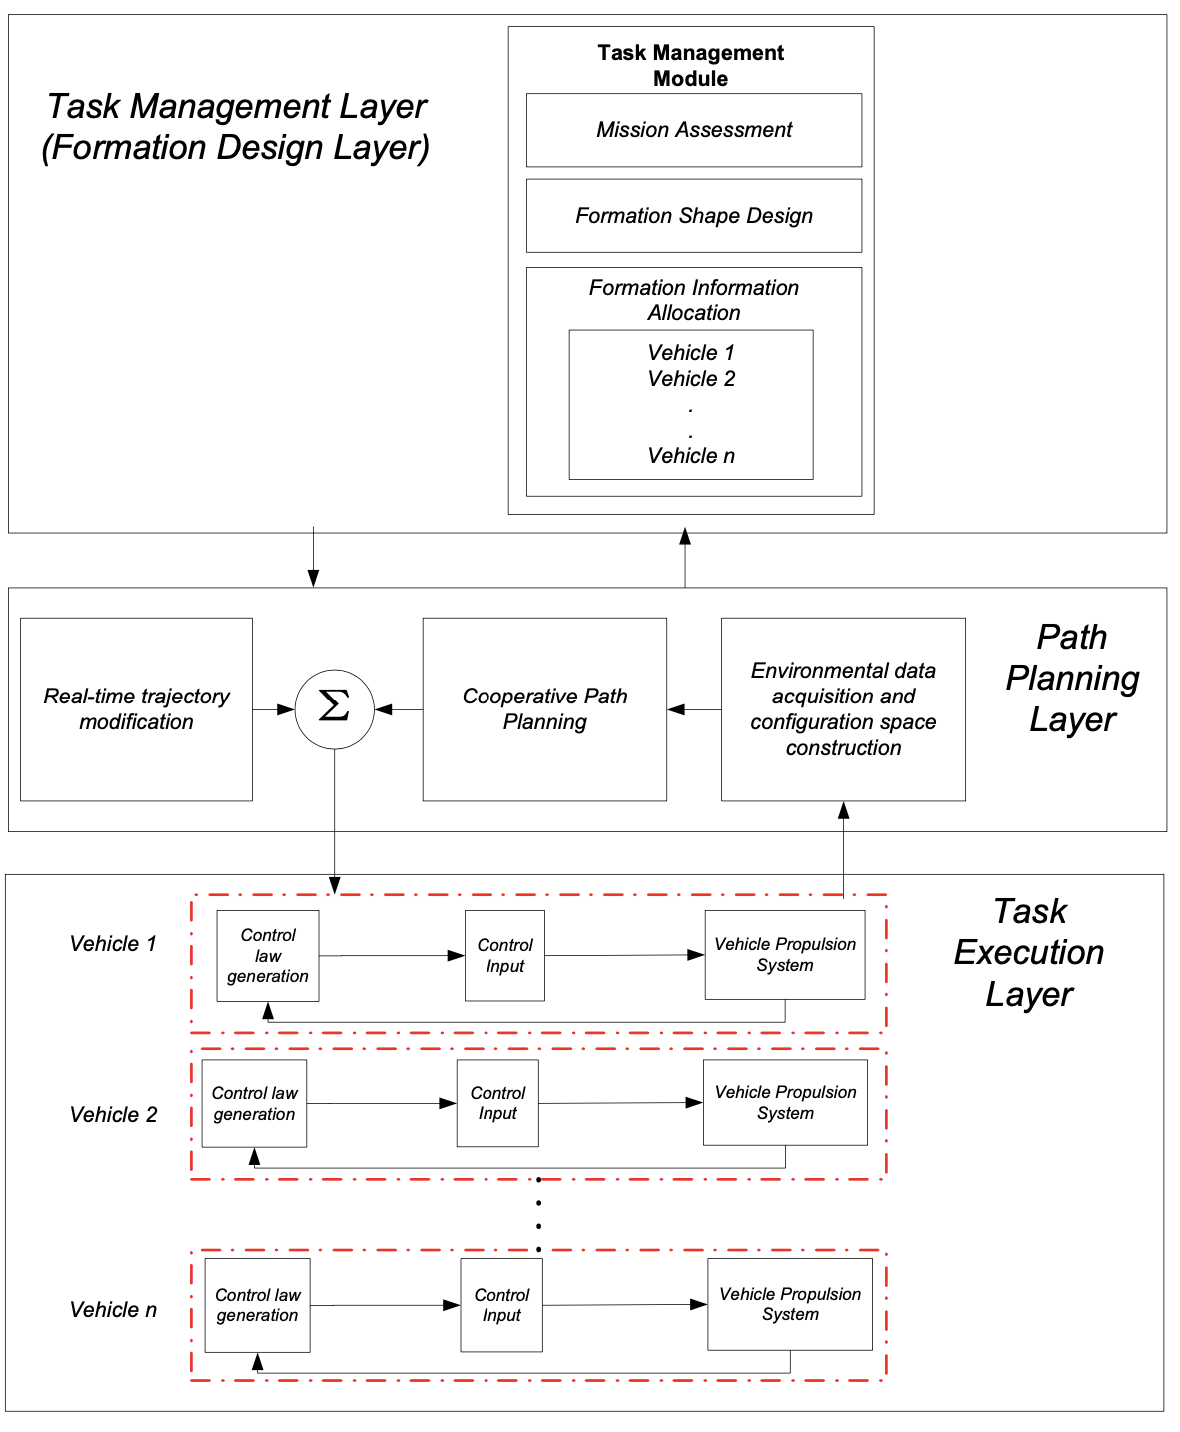
\includegraphics[width=5in]{FormationSystemArchitecture.png}
	\caption{A formationc control architecture.}
	\label{fig:FormationSystemArchitecture} 
\end{figure}

\subsection{System Patterns of Formation}

Based on Campbell et al. \cite{campbell2012review}, as demonstrated in Figure \ref{fig:patternsformation}, four shapes are commonly used:

\begin{compactenum}
	\item Column shape, gives a wide mission area.
	\item Line shape, forms a small mission area but useful in highly constrained environments.
	\item V shape, suitable in normal operations, offers a good view of the surroundings, and easy and direct communication can be eastablished between vehicles.
	\item Diamond shape, a variation of V shape, also frequently used in normal operations.
\end{compactenum}

As mentioned in \cite{liu_bucknall_2018}, there are no particular restrictions on the choice of formation shape. The shape is determined by the task management layer, and should be deformable during tasks, e.g. deform and reform into another shape when trying to enter a narrow area.

In addition, when formation shape change is occurring, the formation control strategy should consider the following additional constraints: 

\begin{compactenum}
	\item Inter-vehicle collision avoidance,
	\item Coordinating of multiple vehicles, i.e. avoid the situation waiting or fully stop due to vehicles lagging behind.
	\item Avoiding deadlock situation, vehicles should not block others' paths.
\end{compactenum}

\begin{figure}
	\centering
	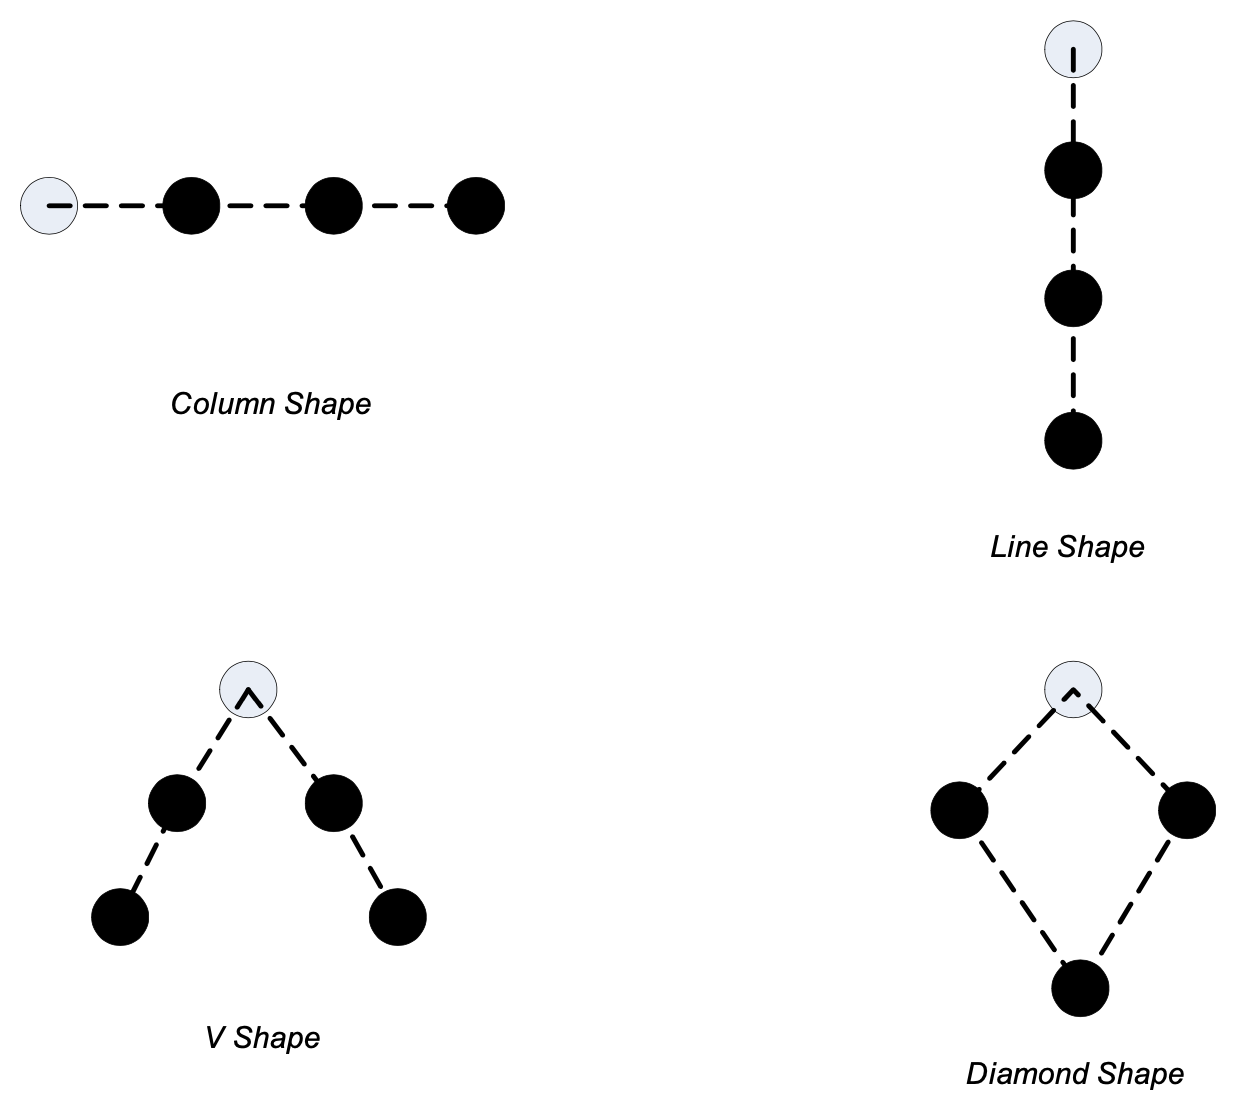
\includegraphics[width=5in]{patternsformation.png}
	\caption{Patterns of formation.}
	\label{fig:patternsformation} 
\end{figure}

\subsection{Review of formation control strategies}

Also as summarised in \cite{liu_bucknall_2018}, there exist three main types of formation maintaince according to different travel scenarios, as displayed in Figure \ref{fig:3typesformationmaintenance}:

\begin{compactenum}
	\item Formation generation and maintenance (Type1), the formation is formed when vehicles are located at random positions with arbitrary headings. Once attained, the shape needs to be maintained to continue the mission.
	\item Formation maintenance during trajectory tracking (Type 2), formation needs to be rigorously maintained while following a predefined trajectory.
	\item Formation shape variation and re-generation (Type 3), the formationshape is maintained as defined in Type2, but the shape also requires adjustment and re-generation while avoiding obsracles.
\end{compactenum}

\begin{figure}
	\centering
	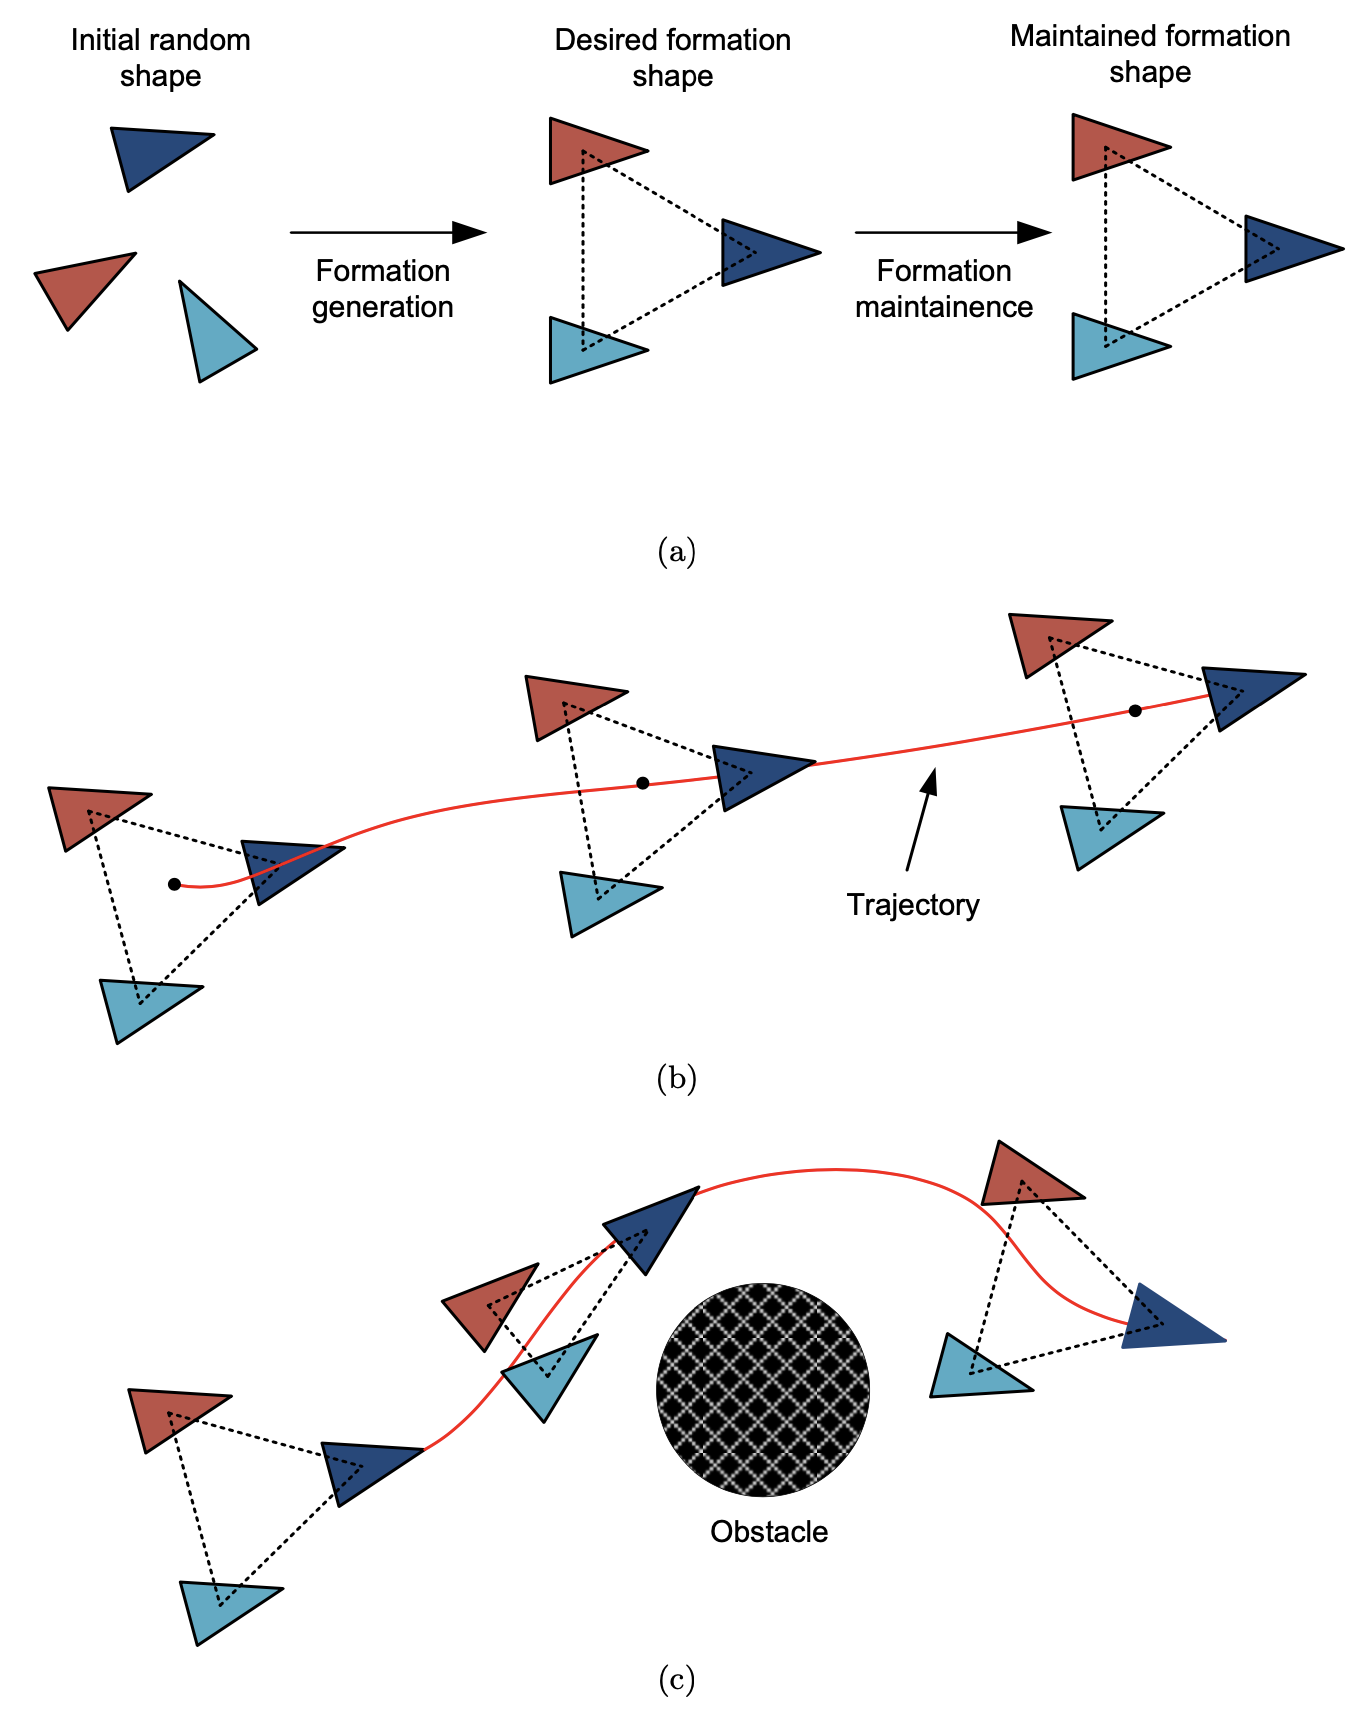
\includegraphics[width=5in]{3typesformationmaintenance.png}
	\caption{Three different types of formation shape maintenance. (a) Formation generation and maintenance. (b) Formation maintenance while tracking trajectory. (c) Formation shape variation and re-generation.}
	\label{fig:3typesformationmaintenance} 
\end{figure}

Three methods have been proposed to achieve formation achieve formation maintenance, 

\begin{compactenum}
	\item leader-follower. One vehicle is regarded as the group leader with full access to the overall navigation information and works as the reference vehicle in the formation. The leader could be virtual in some cases.
	\item virtual structure. In this method, formation shape is treated as a virtual structure or a rigid body. Then the formation is maintained by minimising the position error between the virtual structure and actual formation position.
	\item behaviour-based methods. Control commands are based on various kinds of formation missions e.g. move-to-goal, avoid-static-obstacle, avoid-robot and maintain-formation. And a weight vector are assigned to each kind of command to generate the final control scheme.
\end{compactenum}

Among three methods, leader-follower is the most widely adopted strategy, due to its simple design and implementation. 
While virtual structure method provides better performance in formation maintenance, but with limited capability to deal with collision avoidance since it has no flexibility to adjust the shape. 
The behaviour-based method is most adoptable approach, but lacks system stability analysis, making it unsuitable for large scale utilisation. 
The differences between methods are shown in Figure \ref{fig:diffformationmethods}. 

For future research, a hybrid control strategy appears to be the trend, also fault-tolerant formation control, i.e. capable of dealing with situations when the formation fails.

\begin{figure}
	\centering
	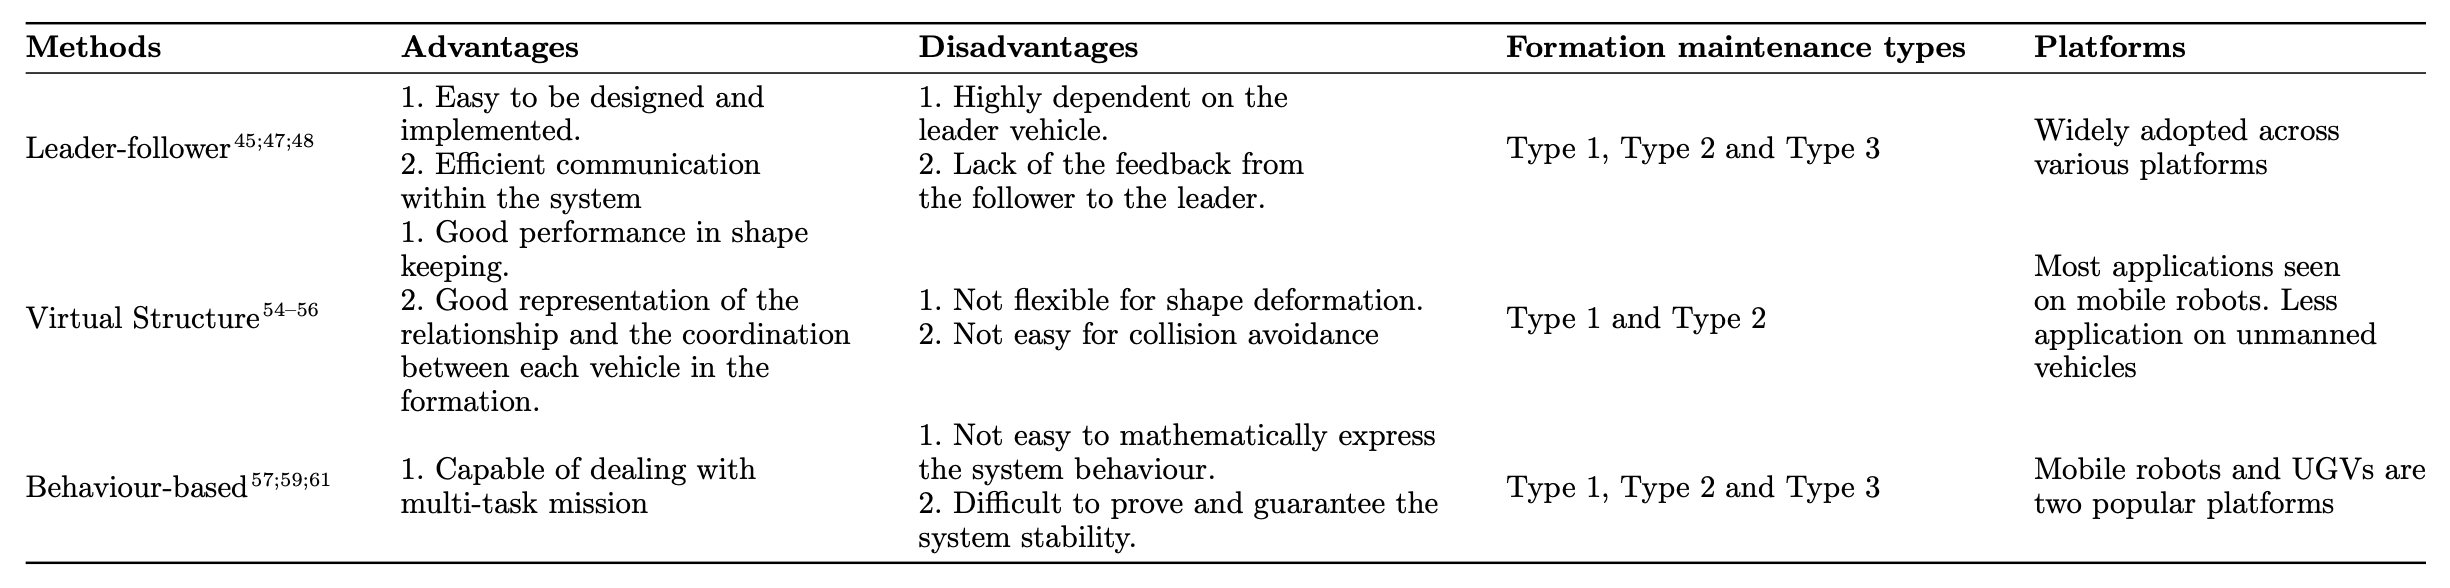
\includegraphics[width=7in]{diffformationmethods.png}
	\caption{Comparison of formation control strategies.}
	\label{fig:diffformationmethods} 
\end{figure}

\section{Cooperative Formation Path Planning}

write this section later.

\begin{figure}
	\centering
	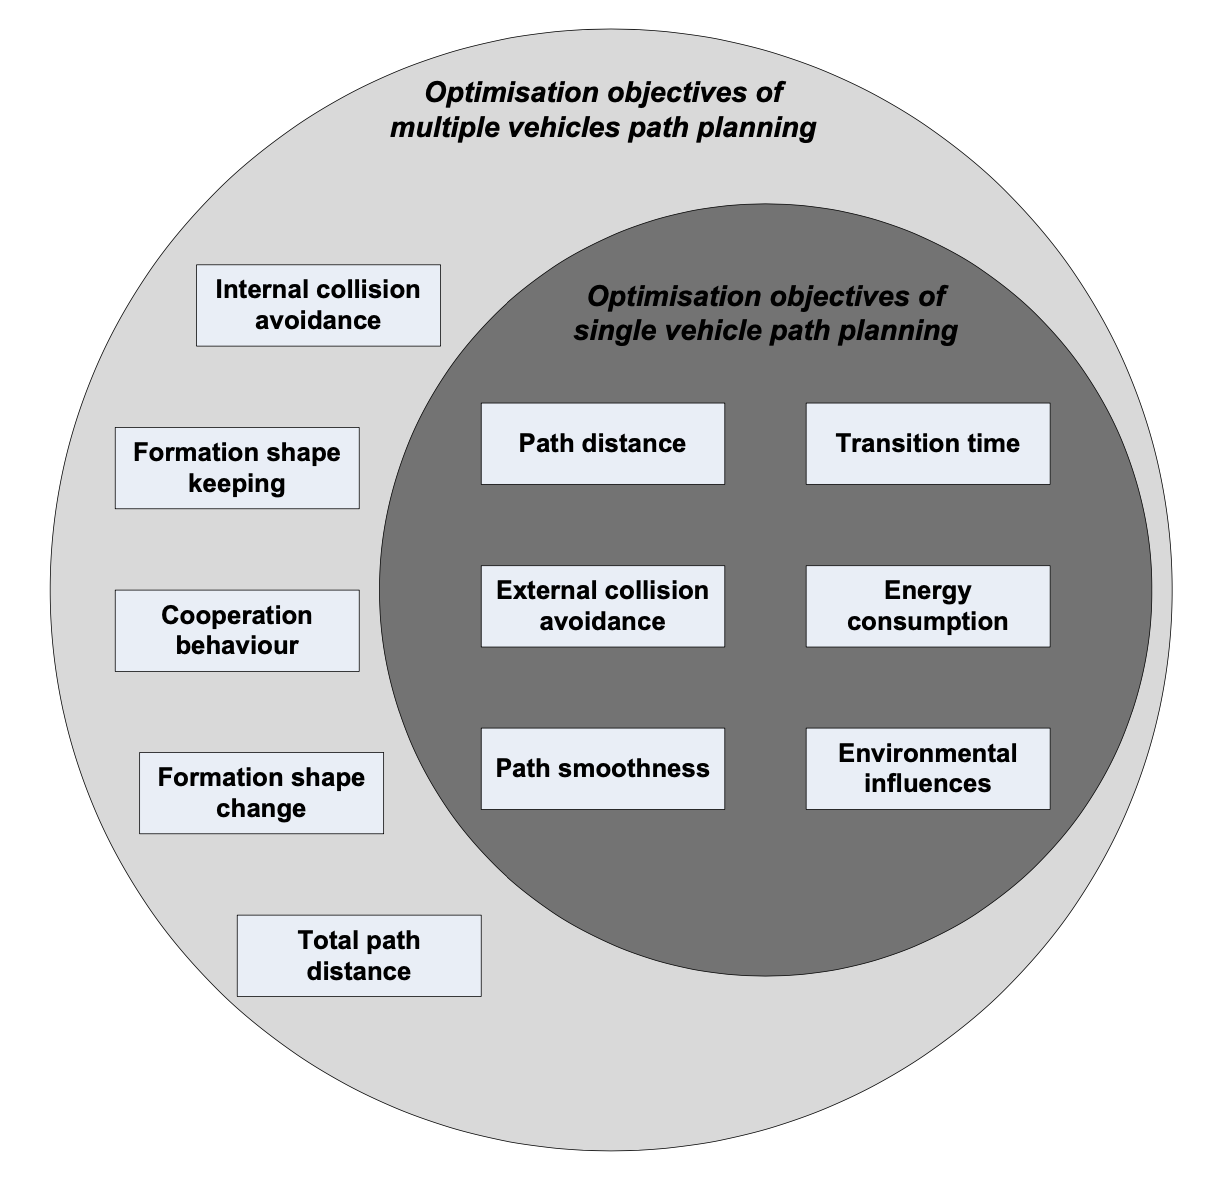
\includegraphics[width=5in]{compsinglemultipathplanning.png}
	\caption{Comparison of optimisation objectives of single and multi agent path planning.}
	\label{fig:compsinglemultipathplanning} 
\end{figure}

\section{Formation Control using Reinforcement Learning}

\subsection{Leader-Follower Fromation using GQ($\lambda$) Reinforcement Learning}

M. Knopp, C. Aykin et al. proposed their method to train a leader-follower formation controller using GQ($\lambda$) reinforcement learning in \cite{knopp2017formation}.

\subsubsection{Framework}

In their work, they train each agent to follow the closest agent in front of it. 
The learning process takes proximity sensors as states and motor speed as action.

They used the GQ$\lambda$ algorithm from Maei and Sutton \cite{maei2010gq} and combined it with an $\epsilon$-greedy behaviour policy to balance between exploration and exploitation.

They build both a simulation using V-REP simulator and a real environment with e-puck robots.

\subsubsection{State Representation}

Their robots have two motors and the speed of each can be set independently to move in 2D, therefore the action space is two-dimensional.
State space also has two dimensions, as the first dimensional the deviation from the optimal distance, and angular error as the second dimension, as shown in Figure \ref{sfig:leaderfollowerrlstate}.
And to reduce ocmputational complexity for deployment on e-puck robots, action and state spaces are discretized with static binary single feature tile coding, in detail, uniform linear tile coding and linear tile coding respectively. 
The tile coding of state space is shown in Figure \ref{sfig:leaderfollowerrltilecoding}.

\begin{figure}
	\centering
	\subfigure[Definition of state space.]{
		\label{sfig:leaderfollowerrlstate}
		\begin{minipage}[t]{0.4\linewidth}
			\centering
			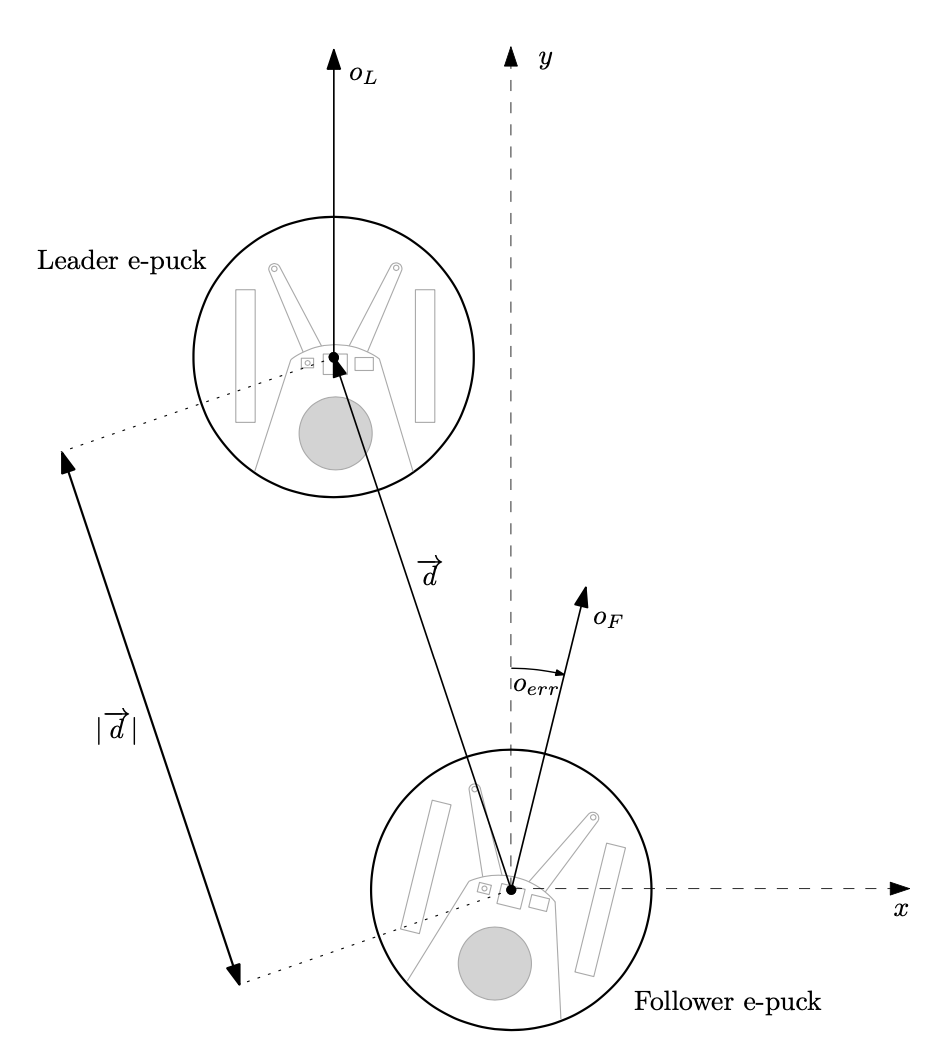
\includegraphics[width=3in]{leaderfollowerrl.png}
			%\caption{fig1}
		\end{minipage}
	}
	\subfigure[9 $\times$ 9 tile coding of state.]{
		\label{sfig:leaderfollowerrltilecoding}
		\begin{minipage}[t]{0.4\linewidth}
			\centering
			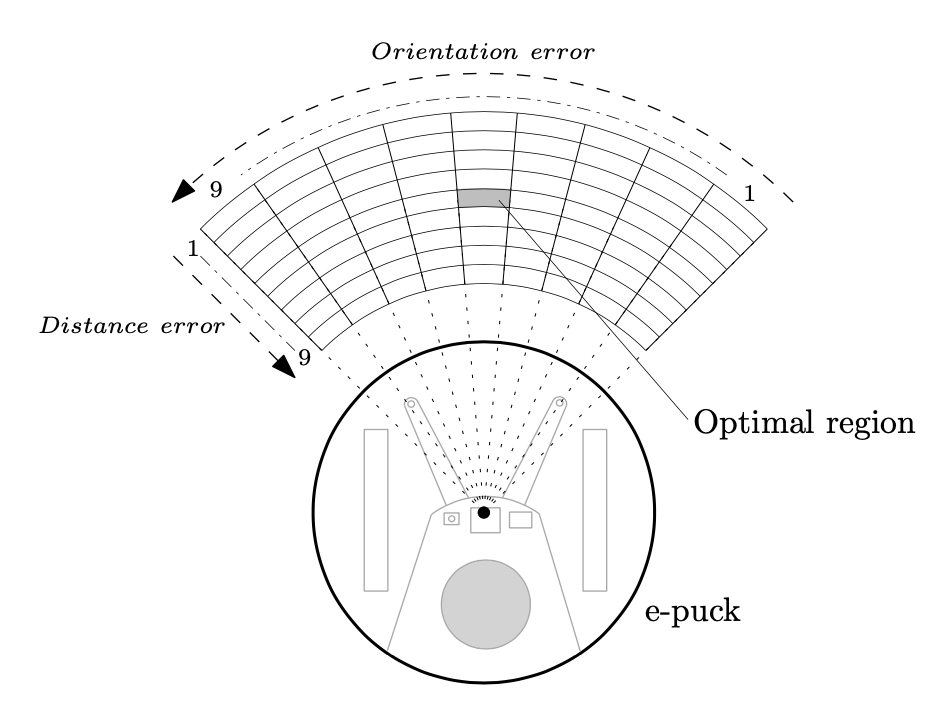
\includegraphics[width=3in]{leaderfollowerrltilecoding.png}
			%\caption{fig2}
		\end{minipage}
	}
	\caption{States and tile coding of leader-follower using RL method.}
	\label{fig:leaderfollowerrl}
\end{figure}

\subsubsection{Reinforcements}

The reinforcement process including its definition of reward function is not clearly stated is their paper.
They might use the two errors in the state to form the reward function, or there might be a specified rewarding principle in the pipeline of GQ$\lambda$ algorithm, which remains to discover.

\subsubsection{Experiment}

In their experiment, the leader agent is programmed to follow a closed circular loop , which is controlled using no learning at all, and the other agents in the group is trained to follow the agent closest in front of them.
They tested their algorithm both in the simulation and real environment.
No quantitative evaluation is provided, but only graphic results, as shown in Figure \ref{fig:leaderfollowerrlresult1} and \ref{fig:leaderfollowerrlresult2}.

\begin{figure}
	\centering
	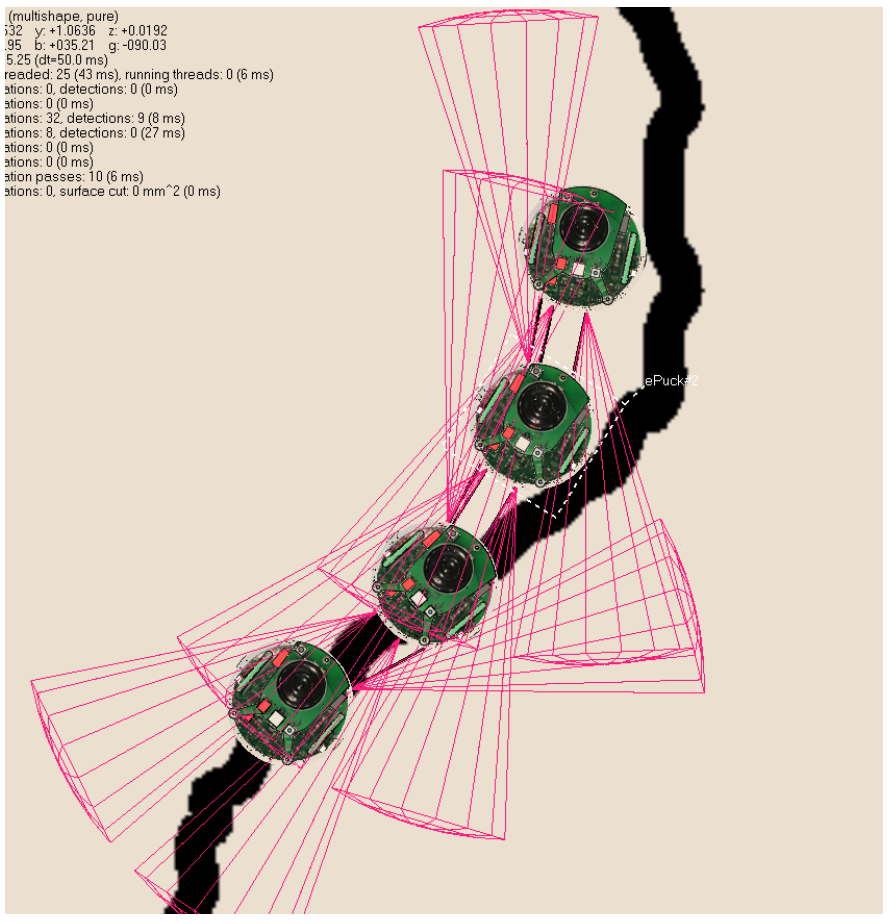
\includegraphics[width=5in]{leaderfollowerrlresult1.png}
	\caption{Simple four agent line formation in V-REP,: the first leader can be found in the lower left corner. The red cones are showing active proximity sensors.}
	\label{fig:leaderfollowerrlresult1} 
\end{figure}

\begin{figure}
	\centering
	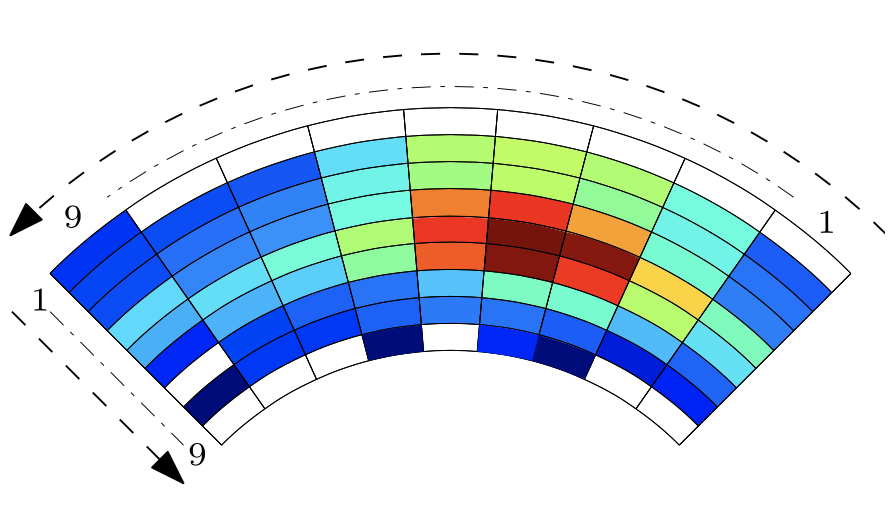
\includegraphics[width=5in]{leaderfollowerlresult2.png}
	\caption{Distribution of visited states at around 1.3 million steps. In 74\% of all cases, the leader was detected in the dark red area right to our optimal region. It stayed within the orange/red 3×3 area on the right side of the optimal region in 98.7\% of the time. To make the rarely visited states discernible, a logarithmic scale is used: red and orange values are in the range of 30\%–1\%, green values are at around 0.1\%, and blue values are another magnitude below that. The non-colored states were never visited in this experiment.}
	\label{fig:leaderfollowerrlresult2} 
\end{figure}

\subsubsection{Discussion}

In this work, the sensor setting is more practical.
Detection of agents in front of the current agents is a well developped technique, which can be done by a variaty of sensors, e.g. lidar or camera.
Also, tile coding is a good method to discretize state and action space.
Some shortcomings can also be summarised:

\begin{compactenum}
	\item This work only explored how to design a leader-follower controller by reinforcement learning, but other formation shapes and maintenance strategy is not considered.
	\item Also, environment obstacles either static or dynamic are ignored.
\end{compactenum}

And they have their research updated in \cite{aykin2018deep}. In this updated work, they use DQN instead of GQ($\lambda$), and take images as input.
\subsection{DRL-enhanced Behaviour-based Method}

In \cite{johns2018intelligent}, R. Johns proposed a method to enhance behaviour-based formationc control with deep reinforcement learning.
In this work, the bahaviour-based method proposed by Balch and Arkin \cite{balch1998behavior} is used as a comparison baseline and also the base from which the reinforment learning algorithms started their training. 

\subsubsection{Framework}

In this method, the reinforment learning network starts with the behaviours of the traditional formation control algorithm, output a action vector $F_{i,rl}$, which is represented as a vector of forces applied to agent $i$ to move.
Then the final control vector $F_{i,control}$ is caculated as a combinition of the behaviour-based control algorithm's force $F_{i,bb}$ and $F_{i,rl}$. 
A single DRL model is used by all agents, as described in the section Parameter Sharing in \cite{johns2018intelligent}, and displayed in Figure \ref{fig:drlbbmparamsharing}.

\begin{figure}
	\centering
	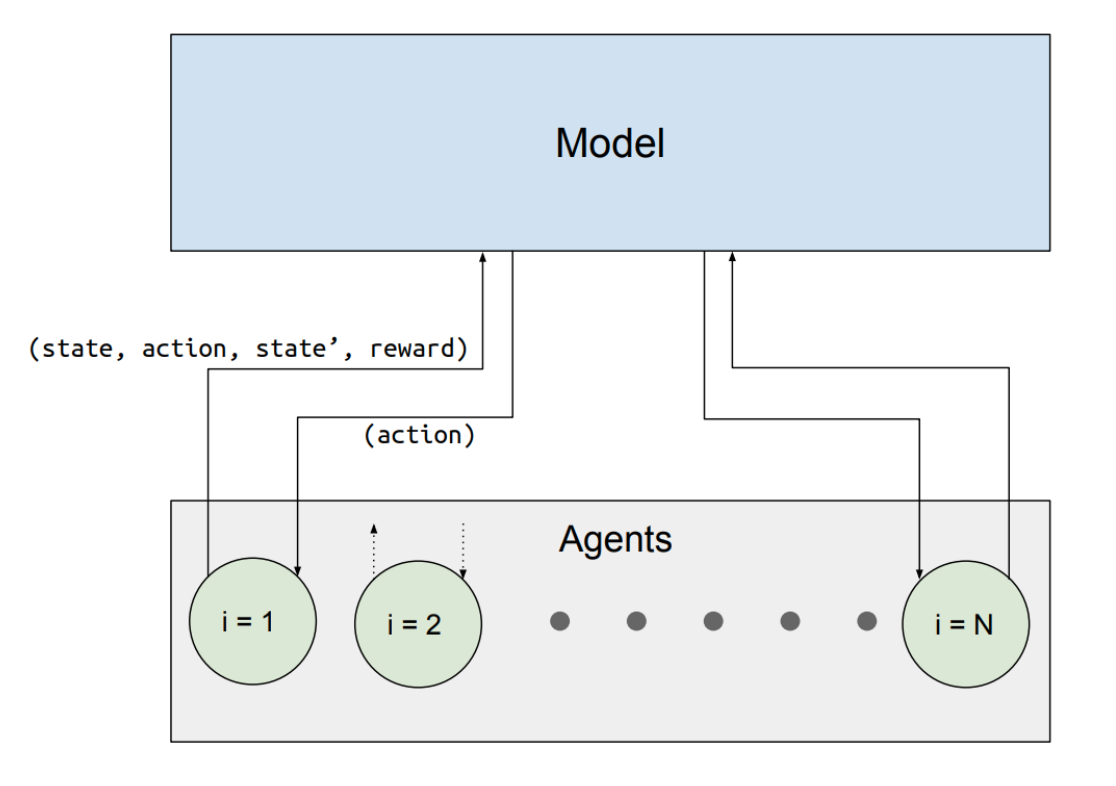
\includegraphics[width=5in]{drlbbmparamsharing.png}
	\caption{The parameter shared DRL model used by all agents.}
	\label{fig:drlbbmparamsharing} 
\end{figure}

The algorithm is implemented using OpenAI's Baselines package \cite{dhariwal2017openai}, which is a set of state-of-the-art Python implementations of reinforcement learning algorithms running on top of Tensorflow.

\subsubsection{State Representation}

In the experiment of this method, each agent is equipped with 8 range sensors, and each lidar sensor is able to recognise if an obstacle or a neighbor agent is being observed. 
And the distance data is converted to sensor power based on a value mapping function as shown in Figure \ref{fig:sensorpower}.

\begin{figure}
	\centering
	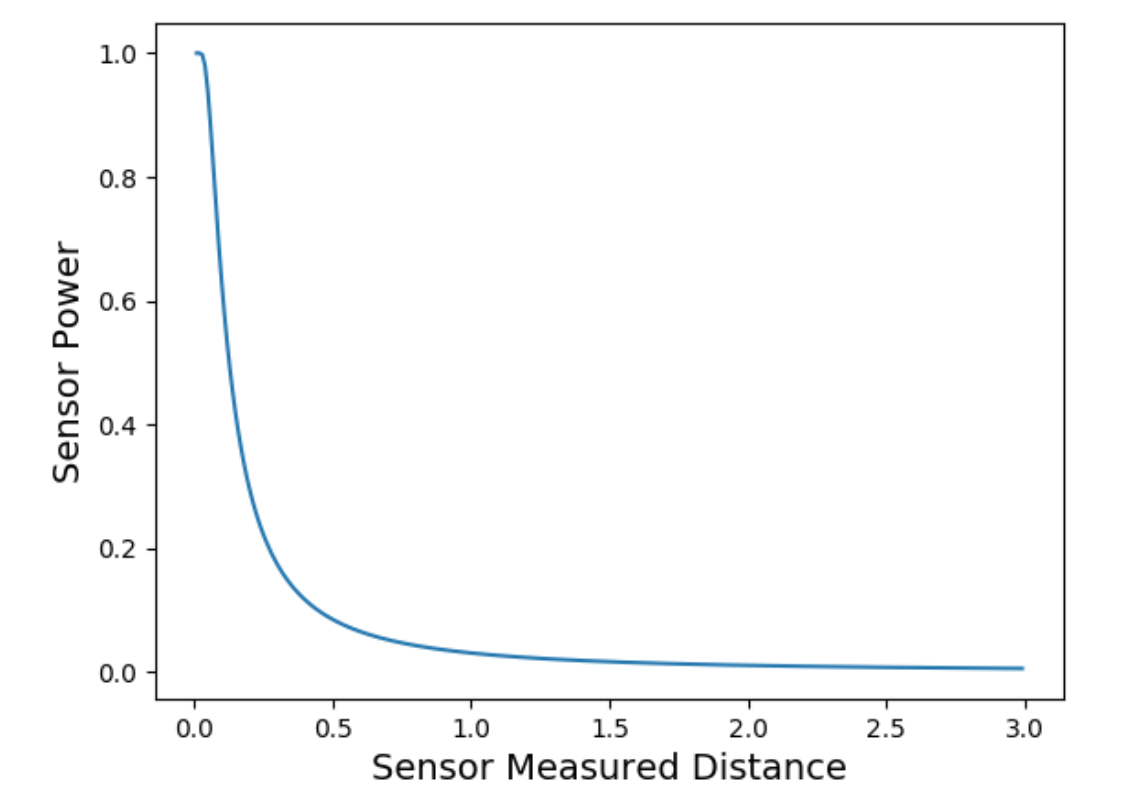
\includegraphics[width=5in]{sensorpower.png}
	\caption{The relationship between the distance measured by a sensor and the sensor’s power in an agents state space.}
	\label{fig:sensorpower} 
\end{figure}

\subsubsection{Reinforcements}

The reward function is composed by four reward parts according to Equation \ref{eq:drlbbreward}.

\begin{equation}
R=R_{ARG}+R_{GRG}+R_{OC}+R_{FD}
\label{eq:drlbbreward}
\end{equation}

\begin{compactenum}
	\item $R_{ARG}$, i.e. Agent Reached Goal, is given to an agent reaching the goal.
	\item $R_{GRG}$, i.e. Group Reached Goal, is awarded to the entire group if one group member reaches the goal.
	\item $R_{OC}$, i.e. Obstacle Collision, added to teach agents to avoid obstacles.
	\item $R_{FD}$, i.e. Formation Displacement, defined as the negative average sum of all agents' formation displacement.
\end{compactenum}

\subsubsection{Experiment}

Expriment is carried on in a 2D simulation map, which is built with the help of OpenAI gym \cite{brockman2016openai}, and obstacles are represented black circles, and agents blue, shown in Figure \ref{fig:drlbbexperiment}.

\begin{figure}
	\centering
	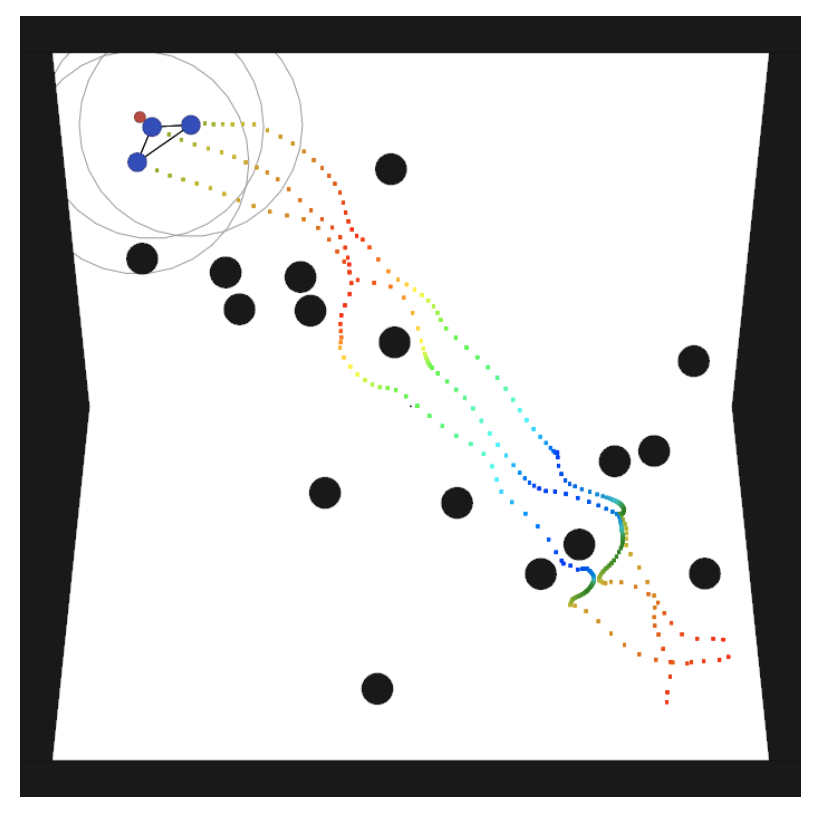
\includegraphics[width=5in]{drlbbexperiment.png}
	\caption{The experiment simulation environment of DRL-enhanced bahaviour-based method.}
	\label{fig:drlbbexperiment} 
\end{figure}

This work also establishes five evaluation metrics:

\begin{compactenum}
	\item Path Ratio. 
	The ratio of the average distance traveled by the agents divided by the Euclidean distance between the start and end point.
	\item Obstacle Collision Frequency. 
	Proportion of time the agents were in contact with an obstacle. 
	A value of zero would imply no agent ever touched an obstacle during the episode, whereas a value of one would indicate that every agent was constantly touching an obstacle during the episode.
	\item Average Formation displacement. 
	A sense of how well the algorithm were at keeping the formation could be established, which is calculated as:
	
	\begin{equation}
		E_{FD}=\frac{1}{TN}\sum_{t=0}^{T}\sum_{n=0}^{N}|x_{n,desired}(t)-x(t)|
	\end{equation}
	
	\item Success. 
	The most important measurement was the percentage of successful attempts to reach the goal. 
	Even if the goal position was not reached in a perfect formation or in the fastest time, the fact that the goal position was reached was considered crucial.
	\item Iterations to Goal. 
	To study how well the agent made use of its ability to move fast, the number of iterations needed to successfully reach the goal was monitored.
\end{compactenum}

The method is tested in 3 experiment stages:

\begin{compactenum}
	\item Fixed Obstacle Positions and Fixed Start and End Positions,
	\item Fixed Obstacle Positions with Random Start and End Positions,
	\item Random Obstacle Positions and Random Start and End Positions.
\end{compactenum}

A sample learning curve is shown in Figure \ref{fig:drlbblearningcurve}, and a sample result table in Figure \ref{fig:drlbbexperimentresult}.

\begin{figure}
	\centering
	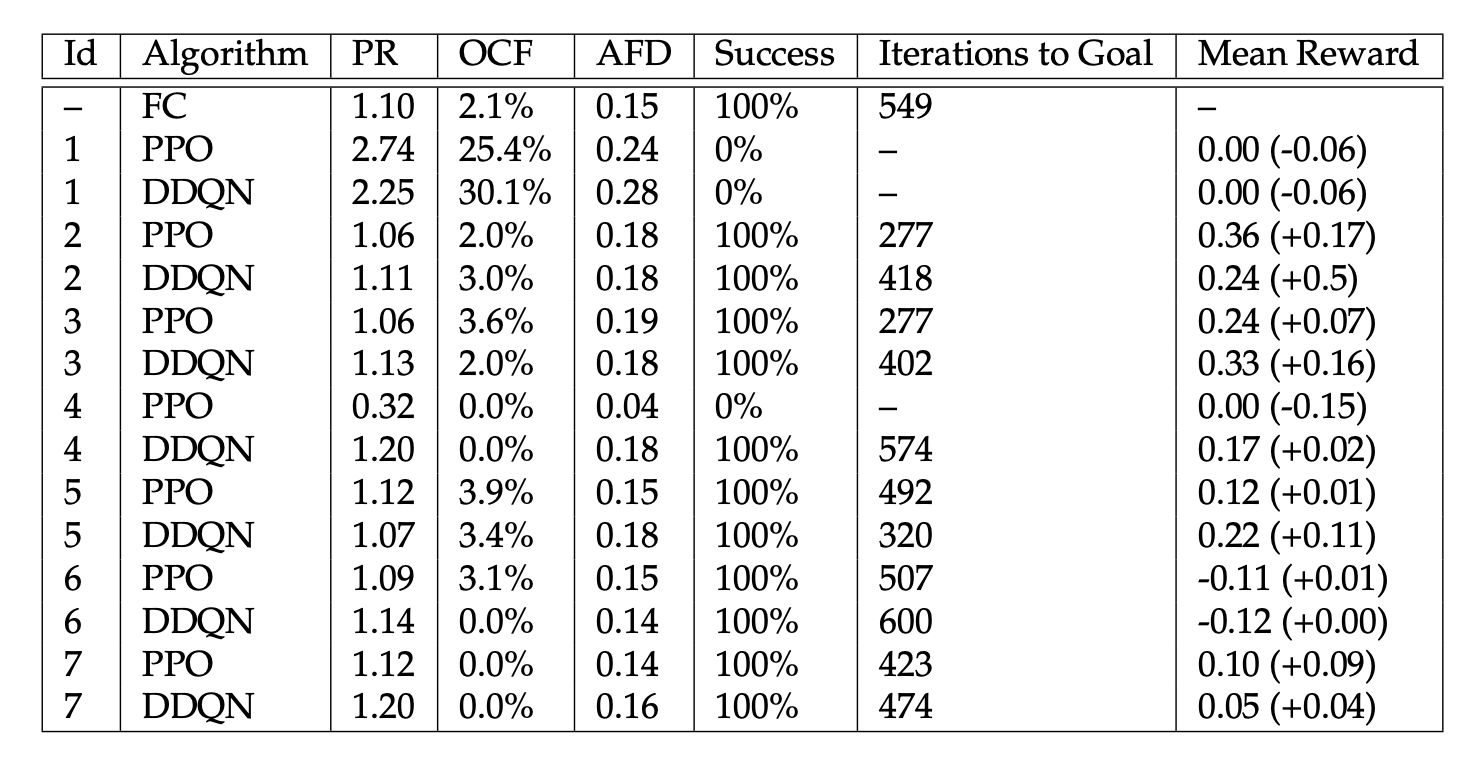
\includegraphics[width=5in]{drlbbexperimentresult.png}
	\caption{A sample result of the experiments of DRL-enhanced Behaviour-based Method.}
	\label{fig:drlbbexperimentresult} 
\end{figure}

\begin{figure}
	\centering
	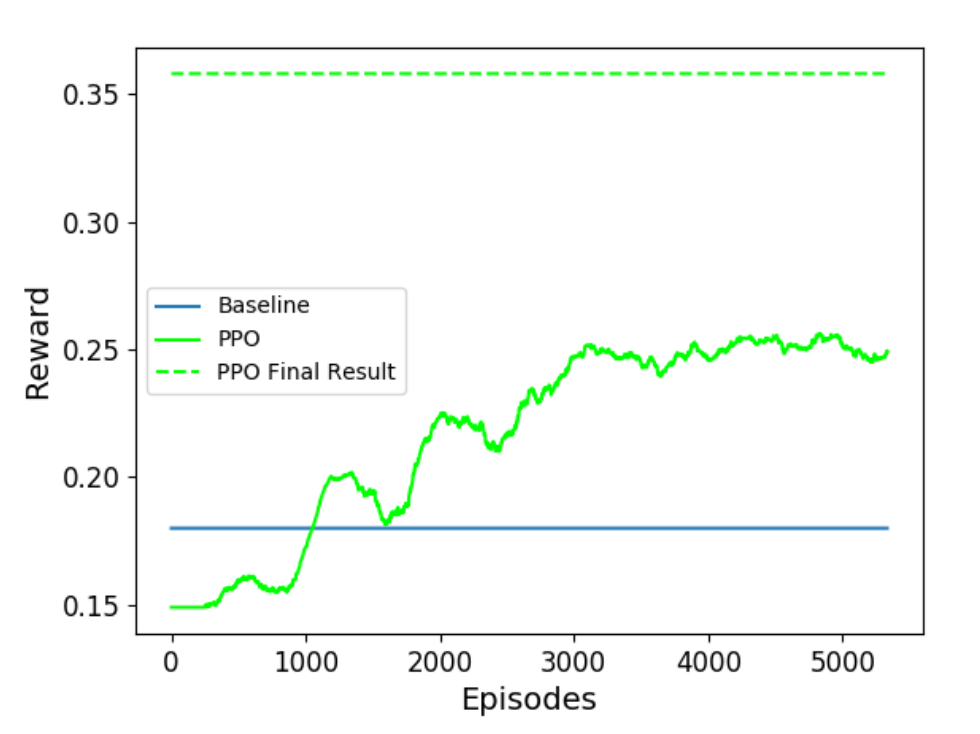
\includegraphics[width=5in]{drlbblearningcurve.png}
	\caption{A sample learning cureve of the experiments of DRL-enhanced Behaviour-based Method.}
	\label{fig:drlbblearningcurve} 
\end{figure}

\subsubsection{Discussion}

This work uses behaviour-based formation control as a base of the training of reinforcement learning network, makeing this method more stable and fast to converge.
A few shortcomings of the method can be concluded:

\begin{compactenum}
	\item The assignment problem is ignored, which means this algorithm has no capability to assign a agent to a new position in the formation during missions, and each agent can only maintain a fixed position, even swithing positions could be more efficient.
	\item The state representation, the set of 8 sensors which can recognise obstacles or neighbor agents, is a set simplified as a simulation and appears to be difficult to realise in a real-world application.
	\item This method employ deep reinforcement learning starting with behaviour-based method, makeing this method easier to train and more practical to apply, but also it introduce extra work to tune the behaviour-based method.
\end{compactenum}


\subsection{Coordinating Formation Control using Reinforcement Learning}

In comparison of the two methods above, A. Rawat and K. Karlapalem \cite{rawat2020multi} proposed another method using reinforcement learning to achive formation control.
The contribution of their method is stated as exploring the formation control problem through a coordination based approach using reinforcement learning, i.e. instead of following a designated leader, agents are detecting neighbor agents and trained to coordinate with them to form a specific formation.

\subsubsection{Framework}

Following the work of the authors in \cite{foerster2018counterfactual, lowe2017multi}, the paradigm of centralized training with decentralized execution is used in this work. 
They use the actor-critic architecture with a central critic as shown in Figure \ref{fig:mobilerobotrlcritic}. 

This central critic  \cite{foerster2018counterfactual} maps the true state of the system and the joint actions taken by the agents at that state to the expected future return. 
The true state of the system is defined as the pose information of all the agents with respect to the centroid of the current formation i.e. $ [x_{i}^{c},y_{i}^{c},\theta_{i}^{c}],\ \forall i \in V $ augmented with the position vector of the goal state with respect to the centroid.
A centralized experience replay is built to store the tuple of past experiences $ <s,r,s',u_{1},...,u_{|A|},o_{1},...,o_{|A|},o'_{1},...,o'_{|A|}>$, $s'$ and $o'$ are the next state of the environment and the observation of each agent in $s'$.
To speed up learning, a experience modifier similar to \cite{andrychowicz2017hindsight} is used to change the goal state to the actual state achived by the agent. 
In this case, the goal is observed with respect to different observation frames and the input to the networks is a sequence containing those goals at different time-steps.

As for actors, each agent has its history of interactions with the environment which it uses to train its policy. The decentralized execution structure is illustrated in Figure \ref{fig:multirobotfcframework}.

\begin{figure}
	\centering
	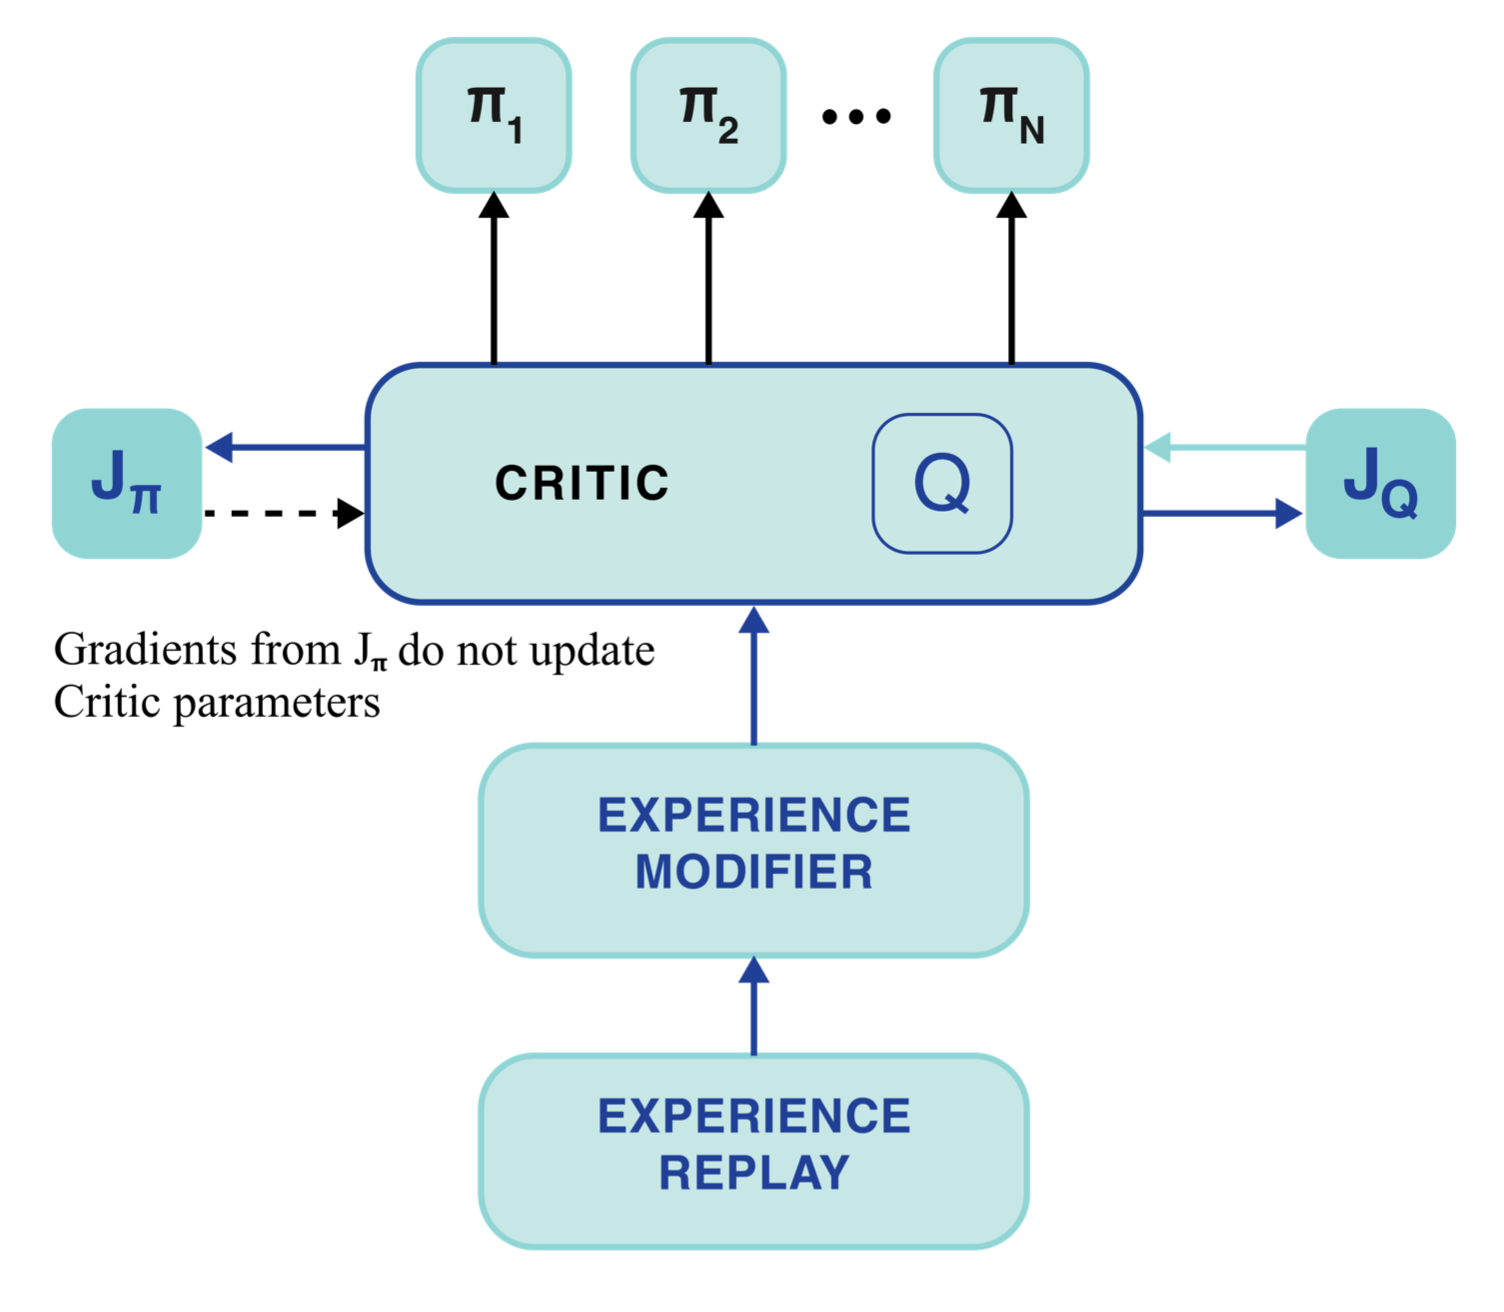
\includegraphics[width=5in]{mobilerobotrlcritic.png}
	\caption{The training involves sampling a batch of experiences, then modifying some of the experiences for positive reinforcement.}
	\label{fig:mobilerobotrlcritic} 
\end{figure}

\begin{figure}
	\centering
	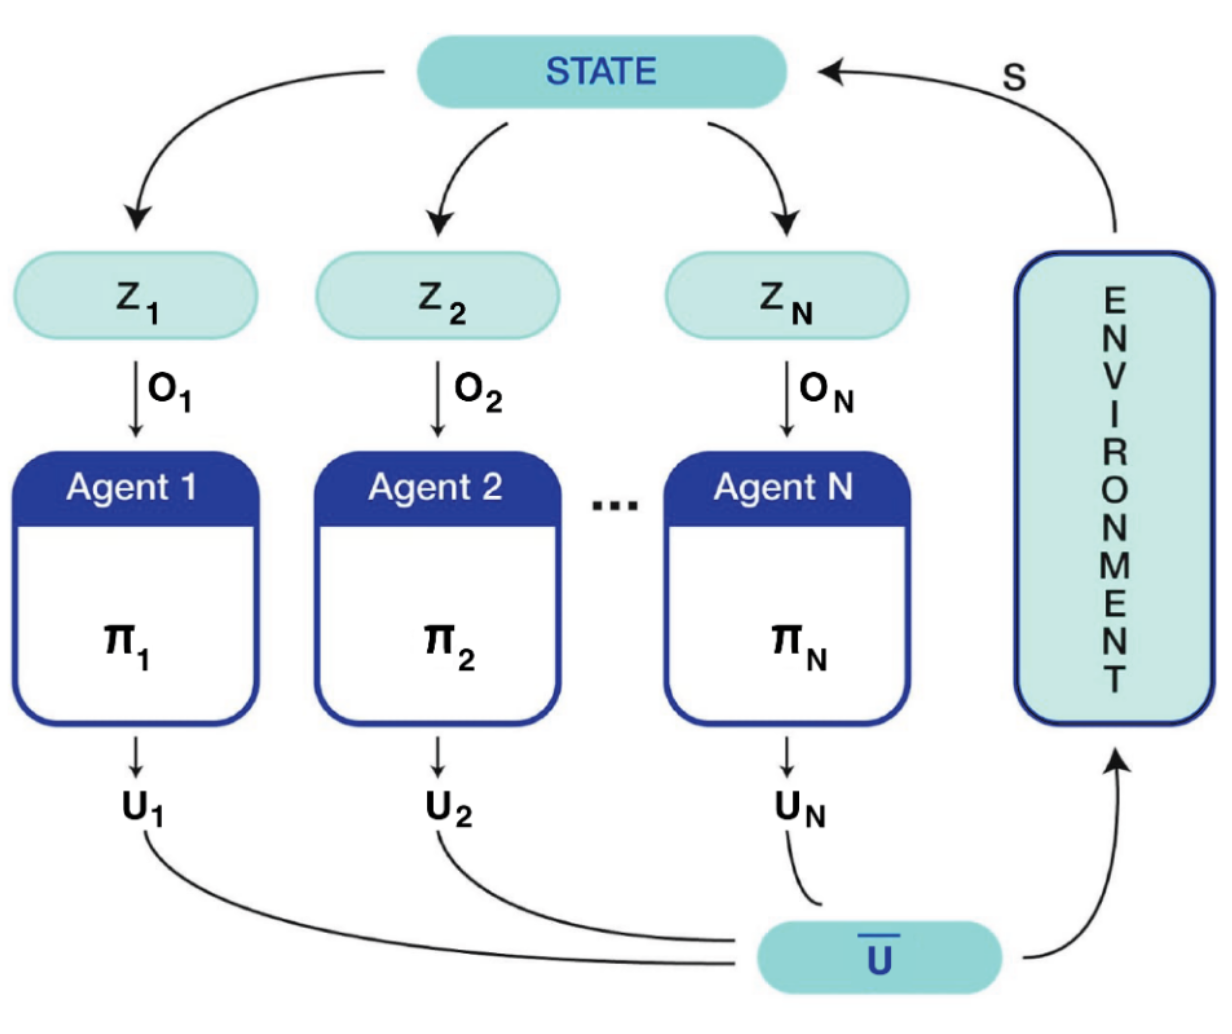
\includegraphics[width=5in]{multirobotfcframework.png}
	\caption{Interaction of agents with the environment. The state of the environment is observed through the observation function $Z_{i}$ of the agent $ i $. The agent acts according to its policy $ \pi_{i} $. The actions of all the agents $ \bar{U} $ transitions the environment to some new state.}
	\label{fig:multirobotfcframework} 
\end{figure}

\subsubsection{State Representation}

They leverage the notion of minimal rigidityand persistent graphs \cite{hendrickx2005rigidity} to define the system.
Each agent is denoted as a vortex $ v_{i} \in V $ in a graph $\mathbb{G} = (V,E) $.
There is a directed edge $e_{i,j}=(v_{i}, v_{j}) \in E$ between two agents $v_{i}, v_{j}$ if and only if agent $v_{i}$ observes agent $v_{j}$.
If each of the agents for any shape of formation observes at least two other agents then a minimally rigid graph is formed.

\subsubsection{Reinforcement}

The agents are rewarded if they are able to maintain the specific distance with the agents that they can observe. 
A reward of greater magnitude is given if the agents are able to reach the goal while maintaining said formation.
Three conditions are introduced as following, to define the reward function:

\begin{compactenum}[C1.]
	\item Formation condition: If all the agents maintain their specified edge lengths within an error of $ \epsilon_{form} $.
	\item Collision condition: This condition is met if the distance between any two agents is less than some threshold (i.e. collision), $ \epsilon_{col} $.
	\item Success condition: If formation condition is satisfied and the centroid of the formation approaches the goal within a threshold distace $ \epsilon_{goal} $.
\end{compactenum}

Then the reward function is defined as:

\begin{equation}
R(s,a,s') = \left\{
	\begin{array}{rcl}
	r_{edge}, & & {if \ only \ C1 \ is \  true}\\
	r_{collision}, & &{if\ C2\  is \  true}\\
	r_{goal}, & &{if\ C3\ is\ true}\\
	r_{penalty}, & &{otherwise}
	\end{array}
\right.
\end{equation}

\subsubsection{Experiment}

The experiment is executed in a custom environment made with the help of OpenAI gym \cite{brockman2016openai}.
The paper illustrated the error in each edge of the formation, and the distance of the centroid from the goal with respect to time for the corresponding trial, as shown in \ref{fig:mobilerobotrlresult}, also the learning curve is shown in Figure \ref{fig:mobilerobotrllearningcurve}.

\begin{figure}
	\centering
	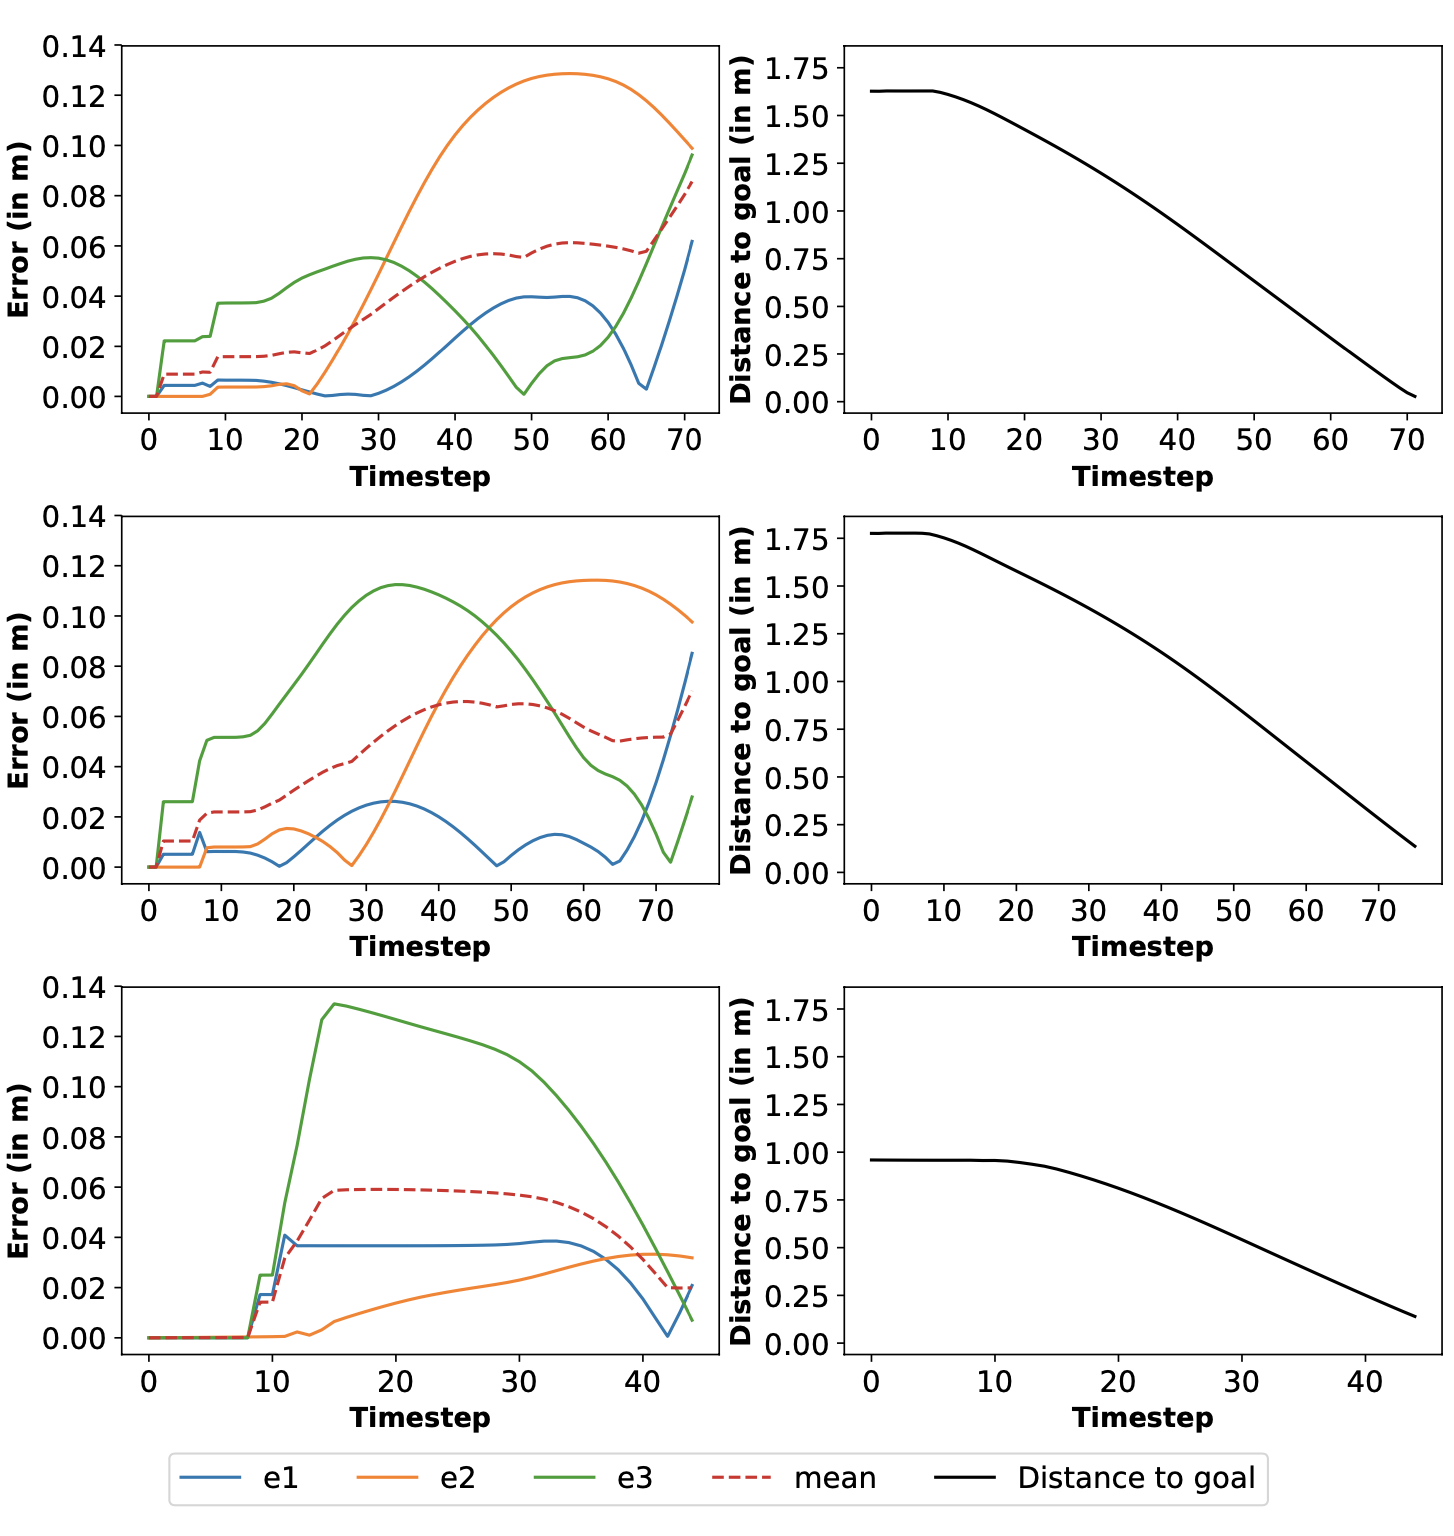
\includegraphics[width=5in]{mobilerobotrlresult.png}
	\caption{The plots on the left show the error in each edge of the formation. The plots on the right show the distance between the centroid of the formation and the goal. The edges between agents are denoted by e1, e2 and e3. The dotted red line denotes the mean error of all the edges.}
	\label{fig:mobilerobotrlresult} 
\end{figure}

\begin{figure}
	\centering
	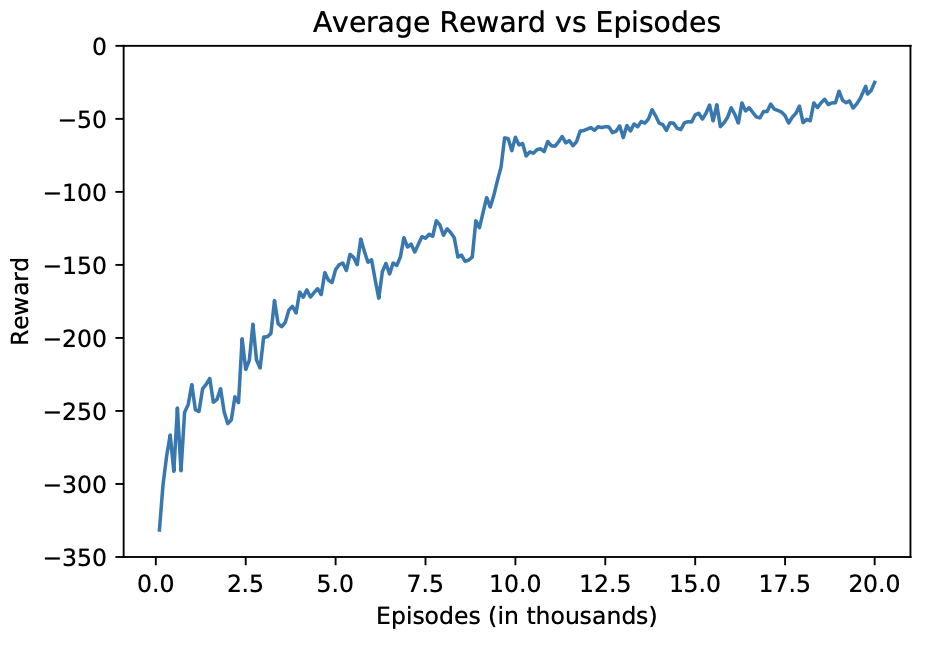
\includegraphics[width=5in]{mobilerobotrllearningcurve.png}
	\caption{Average reward per episode vs. number of training episodes.}
	\label{fig:mobilerobotrllearningcurve} 
\end{figure}

\subsubsection{Discussion}

Compared with the papers reviewed above, this method starts to use the structure of multi-agent reinforcement learning.
The combinition of a centralized critic and decentralized actors is a good application of multi-agent reinforcement learning technique.
Because it uses reinforcement learning for both target reaching and formation control, this method requires less workload to design the controller.
But also shortcomings can be concluded:

\begin{compactenum}
	\item It did not consider the problem of obstacle avoidance,
	\item This method train the deep RL network with no traditional formation control algorithm as a base, so it is suppose to require dramatically more episodes to train until at least a applicable result is attained. But the reward function definitions and full trainnig processes differ significantly between methods reviewed in this article, this possible shortcoming remains for furthur research.
\end{compactenum}


\newpage
\bibliographystyle{ieeetr}
\bibliography{../iVip_ref}

\end{document}
